\documentclass[a4paper,12pt]{article} 
\usepackage[T1]{fontenc}              
\usepackage[frenchb]{babel} % césures, titres français
\usepackage[utf8]{inputenc} % encodage
\usepackage[a4paper,left=3cm,right=3cm,top=2cm,bottom=2cm]{geometry} % marges
\usepackage{graphicx} % insertion d'images
\usepackage{rotating}
\usepackage{float} % permet d'utiliser H pour placer un flottant obligatoirement
\usepackage{pdfpages} % inclusion de PDF au sein du document
\usepackage{listings}
\pagestyle{plain} % pied de pages simples

\setlength{\parskip}{1ex plus 0.5ex minus 0.2ex} % espace entre les paragraphes
\setcounter{tocdepth}{2}
\setcounter{secnumdepth}{2}

\lstset{% general command to set parameter(s)
basicstyle=\ttfamily, % print whole listing small
keywordstyle=\color{black}\bfseries\underbar,
% underlined bold black keywords
identifierstyle=, % nothing happens
commentstyle=\color{white}, % white comments
showstringspaces=false,
numbers=left,
language=java,
breaklines=true,
frame=tblr} % no special string spaces

%%%% debut macro %%%%
\makeatletter
\renewcommand\section{\@startsection {section}{1}{\z@}%
                           {-3.5ex \@plus -1ex \@minus -.2ex}%
                           {2.3ex \@plus.2ex}%
                           {\normalfont\Large\bfseries}}
\makeatother
%%%% fin macro %%%%



% Def
\newcommand{\code}[1]{{\lstinline{#1}}}

\begin{document}
\newpage
\title{J2EE\\TP 3}
\date{}
\author{BRIZAI Olivier\\THORAVAL Maxime}
\maketitle


\section{Utilisation de Spring}
Dans la première partie du TP, nous avons appris à utiliser les bases de Spring. Ce dernier va nous permettre de dissocier, du code Java, 
les classes de service et les DAO. Ceci aura pour effet une plus grande facilité à changer de méthode récupération des données.\\
Par exemple: Nous pourrons décider de passer de l'utilisation d'une base de données à celle de fichiers juste en modifiant un fichier XML 
(en supposant que les classes nécessaires aient été créées au préalable).

\subsection{DAO}
Avant d'utiliser Spring, la récupération d'une classe DAO se faisait de cette manière :
\begin{lstlisting}
	DAOImpl dao = new DAOImpl();
	dao.init();
\end{lstlisting}
Ici, nous avons instancié un objet de type \textit{DAOImpl} et l'avons initialisé.\\
Le principal problème est lié au fait que nous utilisons une classe définie. Si l'on décide de changer le nom du DAO , il faudra modifier le code en conséquence. L'utilisation de Spring va ainsi eviter plusieurs recompilations en cas de changement du DAO. La couche web et le couche service ne seront en effet pas à recompiler.

Voici le nouveau code lorsque l'on utilise Spring :

\begin{lstlisting}
	IDAO dao =(IDAO) (new XmlBeanFactory(new ClassPathResource("spring-config.xml"))).getBean("dao");
\end{lstlisting}

L'identifiant "dao" fait ici appel au bean définie dans le fichier spring-config.xml :

\begin{lstlisting}
<bean id="dao" class="ensicaen.tb.mvc.eleves.dao.DAOImpl" destroy-method="destroy" init-method="init">
</bean>
\end{lstlisting}

Le XML va permettre d'instancier le bean, tandis que c'est le java qui l'utilisera.
On remarque que l'on ignore dans le code java de quelle implémentation du IDAO il s'agit. Ce choix est fait dans le XML et permet de diminuer les dépendances entre les couches.

On vient de mettre en place Spring pour la couche DAO et on fait de même pour la couche service grâce à un bean "service qui représentera une instance de notre classe de service.

Dans le fichier Application.java, on appellera alors l'instance de service ainsi : 

\begin{lstlisting}
service =(IService) (new XmlBeanFactory(new ClassPathResource("spring-config.xml"))).getBean("service");
\end{lstlisting}

On remarque que l'on fait appelle à un IService et non plus à une ServiceImpl, ce qui limite les dépendances (comme pour le DAO).
Notre implémentation d'IService est également défninie dans le fichier spring-config.xml :

\begin{lstlisting}
<!-- La classe Service -->
	<bean id="service" class="ensicaen.tb.mvc.eleves.service.IServiceImpl">
		<property name="dao" ref="dao" />
	</bean>
\end{lstlisting}

On constate qu'elle a comme attribut un "dao", qui fait bien entendu référence au "dao" définit dans le même fichier en XML. Ainsi lorsque l'on
instancie la classe qui gère les service, la classe du DAO sera automatiquement intanciée grâce au XML.

\begin{figure}[H]
	\center
	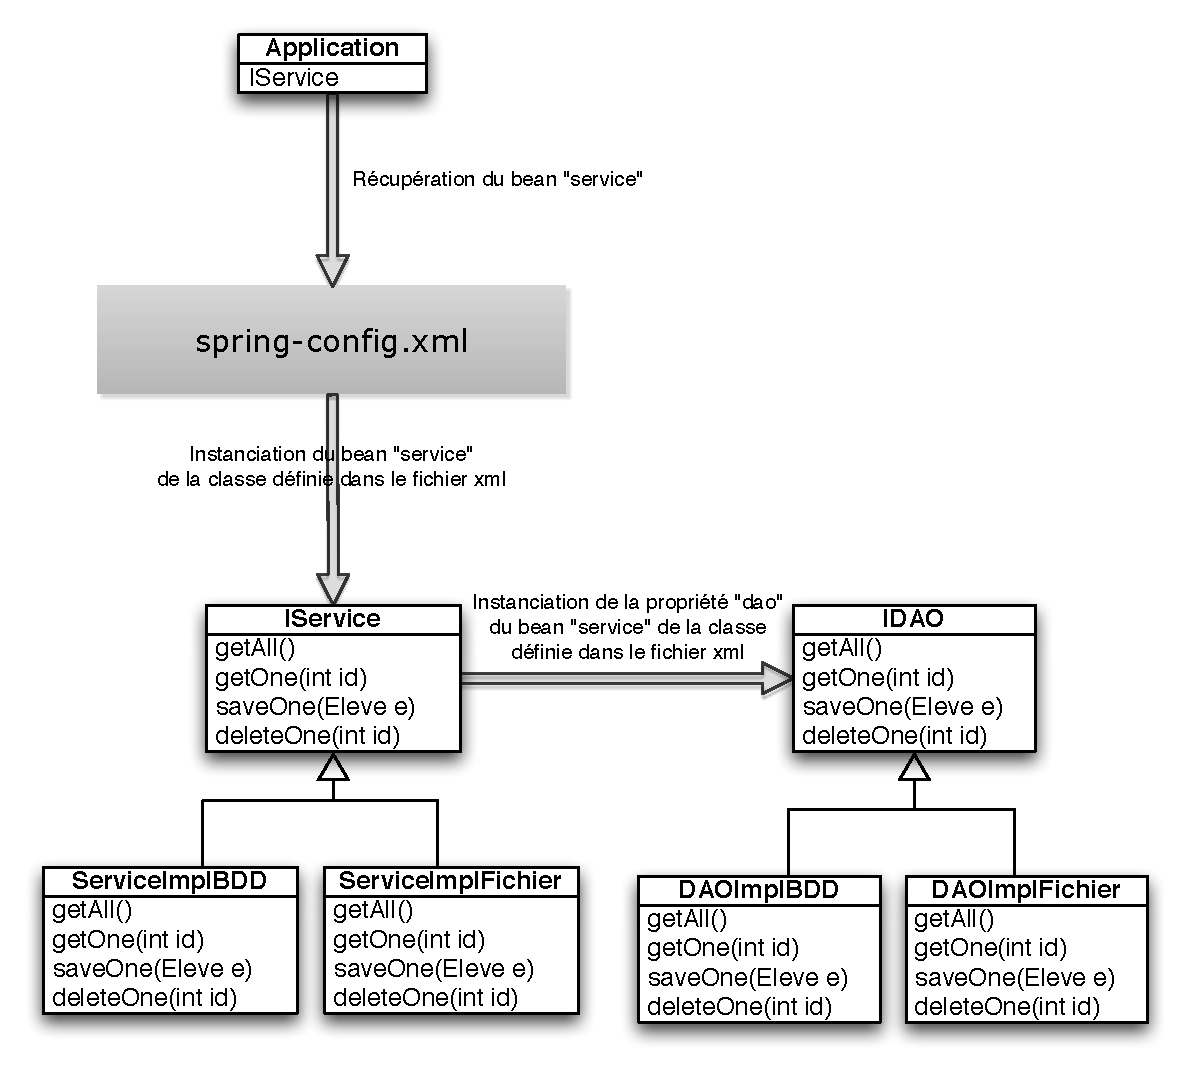
\includegraphics[width=15cm]{img/spring.pdf}
	\caption{Architecture d'utilisation de spring}
\end{figure}
\newpage


\section{Utilisation d'iBatis}

iBatis est une nouvelle couche qui vient s'insérer entre le DAO et la couche d'accès aux données (JDBC).
Dans le fichier spring-config.xml, on va définir de nouveaux Bean. Ces beans vont nous permettre de déporter tous les appels à des fonctionnalitées de 
JDBC du code Java vers le XML.

Si l'on part du coté de la couche d'accès aux données et qu'on remonte vers le DAO, voici les étapes a effectuer dans l'ordre :

Etape 1 : La connection au SGBD est faite dans le bean \textit{dataSource} : 

\begin{lstlisting}
<!-- la source de données utilisant jdbc -->
	<bean id="dataSource"
		class="org.springframework.jdbc.datasource.SingleConnectionDataSource"
		destroy-method="destroy">
		<property name="driverClassName" value="org.postgresql.Driver" />
		<property name="url" value="jdbc:postgresql://postgres/clinique" />
		<property name="username" value="thoraval" />
		<property name="password" value="canari" />
	</bean>
\end{lstlisting}

Etape 2 : On va maintenant définir le fichier XML contenant les informations sur l'architecture de la base de données:

\begin{lstlisting}
<!-- SqlMapClient -->
	<bean id="sqlMapClient" class="org.springframework.orm.ibatis.SqlMapClientFactoryBean">
		<property name="dataSource">
			<ref local="dataSource" />
		</property>
		<property name="configLocation" value="classpath:sql-map-config-postgres.xml" />
	</bean>
\end{lstlisting}

On remarque que ce bean est lié au Bean précédent \textit{dataSource}, en effet l'accès aux données requiert une connexion au SGDB.

Etape 3 : L'étape située en amont de l'accès aux données, c'est la définition du bean du DAO. Ce bean est lié au bean \textit{sqlMapClient} précédent
à travers lequel il va effectuer ses requêtes sur la base de données.

\begin{lstlisting}
<!-- La classe DAO -->
	<bean id="dao" class="ensicaen.tb.mvc.eleves.dao.DAOImplCommon">
		<property name="sqlMapClient" ref="sqlMapClient" />
	</bean>
\end{lstlisting}

Comme on le voit ici, on a définit pour l'occasion un nouveau DAO en java : \textit{DAOImplCommon}

\begin{lstlisting}
public class DAOImplCommon extends SqlMapClientDaoSupport implements IDAO {
\end{lstlisting}

Il remplace la précédente classe DAOImpl.
Il implémente naturellement l'interface IDAO, mais surtout il hérite de SqlMapClientSupport qui est une classe de la bibliothèque iBatis.


Le fichier  \textit{sql-map-config-postgres.xml} permet de "mapper" nos classes métiers à des tables de la base de données.
\textit{sqlMapClient}. 

\begin{lstlisting}
<sqlMapConfig>
	<sqlMap resource="eleve-postgres.xml" />
</sqlMapConfig>
\end{lstlisting}

Dans \textit{sql-map-config-postgres.xml} on a renseigné le fichier \textit{eleve-postgres.xml}. Dans ce fichier est défini le mapping de classe Eleve avec une table associée dans la base de donnée. Ce mapping va permettre à iBatis d'instancier un bean de type Eleve à partir des informations de la base de données, tout cela sans que le développeur n'est à intervenir. De plus, une insertion dans la base d'un Eleve va automatiquement mettre l'objet avec l'id généré.
On a ainsi déporté toute la partie JDBC au sein de fichier XML.

\begin{lstlisting}
<?xml version="1.0" encoding="UTF-8"?>

<!DOCTYPE sqlMap PUBLIC "-//ibatis.apache.org//DTD SQL Map 2.0//EN"
	"http://ibatis.apache.org/dtd/sql-map-2.dtd">
	
<sqlMap>
	<!--  alias classe [Eleve] -->
	<typeAlias alias="Eleve.classe" type = "ensicaen.tb.mvc.eleves.entities.Eleve"/>
	
	<!--  mapping table [ELEVES] -objet [Eleve] -->
	<resultMap id="Eleve.map" class="Eleve.classe">
		<result property="id" column="id"/>
		<result property="version" column="version"/>
		<result property="nom" column="nom"/>
		<result property="prenom" column="prenom"/>
		<result property="dateNaissance" column="datenaissance"/>
		<result property="redoublant" column="redoublant"/>
		<result property="annee" column="annee"/>
		<result property="filiere" column="filiere"/>		
	</resultMap>
	
	<!--  liste de tous les eleves -->
	<select id="Eleve.getAll" resultMap="Eleve.map">
		SELECT * FROM ELEVES
	</select>
	
	<!--  obtenir un eleve en particulier  -->
	<select id="Eleve.getOne" parameterClass="int" resultMap="Eleve.map">
		SELECT * FROM ELEVES WHERE id=#value#
	</select>
	
	<select id="Eleve.nbEleve" resultClass="int">
		SELECT count(*) FROM ELEVES
	</select>
	
	<!-- ajouter un eleve -->
	<insert id="Eleve.insertionOne" parameterClass="Eleve.classe">
		<selectKey keyProperty="id">
			SELECT nextval('SEQ_ELEVES') as value
		</selectKey>
		INSERT INTO ELEVES values (#id#, 1, #nom# , #prenom#, #dateNaissance#, #redoublant#, #annee#, #filiere#)
	</insert>
	
	<!-- mettre à jour un élève -->
	<update id="Eleve.updateOne" parameterClass="Eleve.classe">
		UPDATE ELEVES SET version = #version#, nom = #nom#, prenom = #prenom#, dateNaissance = #dateNaissance#,
		 annee = #annee#, redoublant = #redoublant#, filiere = #filiere# WHERE id = #id#
	</update>
	
	<!-- supprimer un élève -->
	<delete id="Eleve.deleteOne" parameterClass="int">
		DELETE FROM ELEVES WHERE id = #id#
	</delete>

</sqlMap>
\end{lstlisting}

L'appel aux fonctions de cette classe Eleve, se feront comme précédemment dans le DAO, en l'occurance ici dans la classe \textit{DaoImplCommon}.
En revanche l'appel est ici transparent puisque l'accès à la BDD est géré dans le XML :
Voici un exemple pour la suppression d'un élève :

\begin{lstlisting}
public void deleteOne(int id) {
		try {
			getSqlMapClientTemplate().delete("Eleve.deleteOne",id);
		} catch (Exception ex) {
			throw new DAOException("Delete impossible \n" + ex.getMessage(), 50);
		}
}
\end{lstlisting}

Comme précédemment, pour diminuer le couplage, l'implémentation de la couche service est définie dans le fichier \textit{spring-config.xml} :

\begin{lstlisting}
<bean id="service"
		class="org.springframework.transaction.interceptor.TransactionProxyFactoryBean">
		<property name="transactionManager" ref="transactionManager" />
		<property name="target">
			<bean class="ensicaen.tb.mvc.eleves.service.IServiceImpl">
				<property name="dao" ref="dao" />
			</bean>
		</property>
		<property name="transactionAttributes">
			<props>
				<prop key="saveMany">PROPAGATION_REQUIRED</prop>
				<prop key="deleteMany">PROPAGATION_REQUIRED</prop>
			</props>
		</property>
	</bean>
\end{lstlisting}

Ici aussi l'instanciation de la classe de service provoque l'instanciation de la classe du DAO. (rajouter un comentaire sur les transactions)

Voici un schéma qui résume un peu plus clairement ce qui a été dit :

\begin{figure}[H]
	\center
	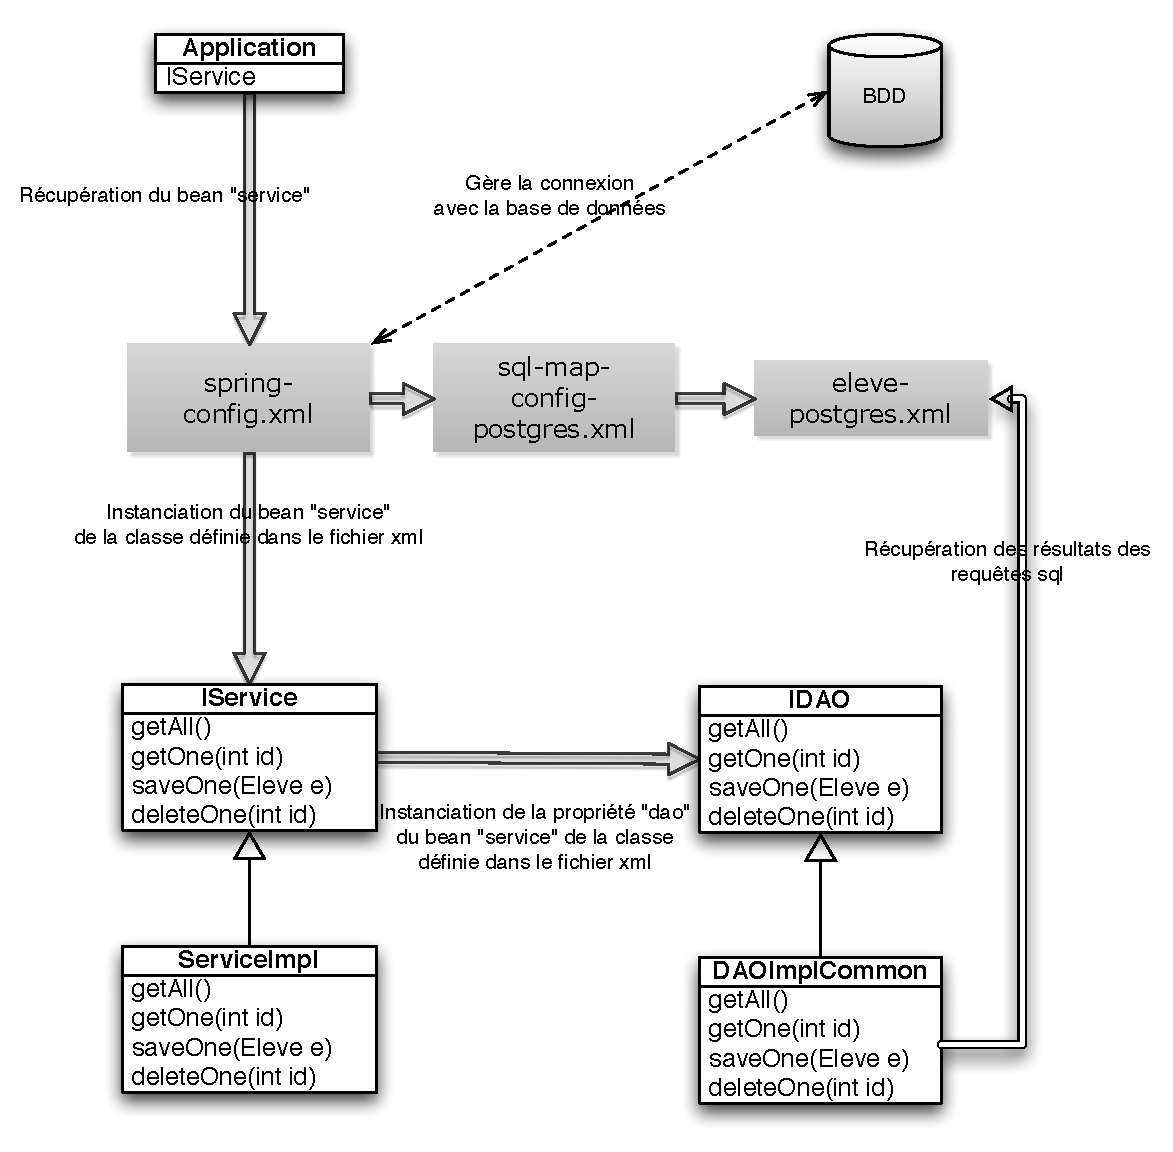
\includegraphics[width=15cm]{img/springibatis.pdf}
	\caption{Architecture d'utilisation de spring avec ibatis}
\end{figure}

\newpage

\end{document}




